\documentclass[11pt,a4paper]{article}
\renewcommand{\baselinestretch}{1.05}

\usepackage{amsbsy,amstext,amsmath,graphicx}

\usepackage[dvipdfm]{color}
\definecolor{darkred}{rgb}{0.8,0,0}

\newcommand{\bs}{\boldsymbol}
\newcommand{\nuc}[2]{\mbox{$^{#1}$#2}}

\addtolength{\textwidth}{3cm}
\addtolength{\oddsidemargin}{-1.5cm}
\addtolength{\evensidemargin}{-1.5cm}
\addtolength{\textheight}{2\baselineskip}
\addtolength{\topmargin}{-\baselineskip}

\renewcommand{\descriptionlabel}[1]{\hspace\labelsep\normalfont\ttfamily #1}
\newcommand{\sys}{{\tt spin\_system}}
\newcommand{\cmx}{{\tt cmatrix}}
\newcommand{\rmx}{{\tt rmatrix}}
\newcommand{\llist}{{\tt ListList<T>}}
\newcommand{\spacet}{{\tt space\_T}}
\newcommand{\cvector}{{\tt List<complex>}}
\newcommand{\rvector}{{\tt List<double>}}
\newcommand{\libname}{{\tt libcmatrix}}
\newcommand{\ket}[1]{\ensuremath{\langle #1 \rangle}}
\newcommand{\eq}[1]{Eqn.~(\ref{#1})}
\newcommand{\lp}{\hspace{2em}}
\newcommand{\indexheader}[2]{{\tt #1}\index{#2@{\tt #1}}}

\usepackage[colorlinks=true,linkcolor=darkred,dvipdfm]{hyperref}
%\usepackage[colorlinks=true]{hyperref}

\begin{document}

\begin{center}
\Large {\tt crystal} module of {\tt libcmatrix}\\
\large (experimental version)
\end{center}

This code provides a way to generate Hamiltonians and spin operators
for spin systems with permutation symmetry, in particular resulting
from translational symmetry.

Existing \libname\ functions can be used
to calculate operators in the conventional Zeeman eigenbasis that can then be
block-diagonalised by unitary transformations by matrices of the form
\begin{equation}
\begin{pmatrix}
1 & 1 & 1 & \dots \\
1 & e^{2\pi i/n} & e^{4\pi i/n} & \dots \\
\vdots & \vdots & \ddots & 
\end{pmatrix}
\label{Vmatrix}
\end{equation}
where $n$ is the number of states in a set linked by permutation.
$n$ is necessarily a factor of $N$---the number of spins being permuted.
This approach is adequate for small problems, but is unsuited to large 
problems.  Most importantly, it doesn't allow larger spin systems
to be studied.

A better solution is to calculate the spin operators etc.\
directly in the symmetrised basis.  The resulting matrices are smaller
by a factor of $\sim N$, allowing for much more efficient calculation
(by a factor of $N^2$) for a given $N$, or larger problems
to be solved.  Although only an extra $\log_2 N$ spin-1/2 spins can
be added, the efficiency savings do make calculations on large
(say $>10$) spins a realistic possibility.

There are limitations to the current implementation:
\begin{itemize}
\item Limited to spin-1/2.  Extension to other spin quantum numbers
or mixed spin systems would not be too difficult, but is of relatively
little interest.  Large spin systems are only relevant to strongly
coupled systems, which is rarely an issue outside of spin-1/2 NMR\@.
The existing {\tt libcmatrix} functions can be used here in any case.

\item Limited to cyclic permutations of all spins, corresponding
to one-dimensional translational symmetry (with periodic boundary).
The restriction to one dimension of translational symmetry
is a major one.  Adding additional \emph{point} group symmetries
e.g.\ mirror planes, is not particularly useful since additional
block diagonalisation is restricted to ``special'' values of the
translational eigenvalue, $k$, notably $k=0$.  
Adding ``independent'' symmetries such as additional translational
axes would be useful.  This would require some major addition to the
code (effectively all the functions would take on forms that
handled two, three etc.\ $k$ eigenvalues), but is not impossible.
Unfortunately the size of problem that
could be considered is small, even for just 2 dimensions, and may not be sufficient to be
convincing.

\item Only one level of ``$m_z$ blocking'' is supported.  Under free precession,
$m_z$ is a good quantum number for each nucleus type (high-field approximation).
In this case, blocking is limited to the \emph{total} $m_z$, or to one nucleus
type.

\item Although the functions are intended to resemble existing
functions closely, a perfect match
(e.g.\ having a {\tt periodicspin\_system} that ``looked''
like a {\tt spin\_system}) is impossible.  Code that uses
these functions will always be signficantly more involved.

\end{itemize}


\section{Setting up the problem}

Two data objects are declared in {\tt crystal.h}; {\tt CrystalSpec}
``specifies'' the symmetry by declaring which spin states are
related by symmetry.  Adding different permutation symmetries
other than 1D translational is a matter of generating the correct
{\tt CrystalSpec}, but is still restricted to a single ``eigenvalue''.
{\tt CrystalSystem} then uses the information from a {\tt CrystalSpec} object to
create spin operators.  A {\tt CrystalSpec} is initialised using 
\begin{description}
\item[CrystalSpec(spinhalf\_system {\it sys},$N$,bool {\it mzblock},{\it neigs})] creates 
the ``symmetry specification'' for $N$ cells of a given system of spin-1/2 spins.  The {\it mzblock}
flag should be {\tt true} if the states will be blocked by $m_z$ quantum
number i.e.\ free-precession problems, or not.  {\it neigs} is the number
of ``active'' eigenvalues; typical values are $N$ (also the default if omitted),
or $(N+1)/2$ which corresponds to positive values of $k$ only (the translational
eigenstates are numbered 0 to $N-1$ where $N-1$ corresponds to $k=-2\pi/N$ etc.).
Note that the optional $m_z$ blocking is via the {\emph total} $m_z$ quantum number
which will not be appropriate for all heteronuclear problems. 
\item[CrystalSpec(spinhalf\_system {\it sys},$N$,char* {\it label},{\it neigs})] allows a system
to be blocked by $m_z$ of a chosen nucleus e.g. {\tt "13C"} etc.  This is necessary
if $m_z$ is only a good quantum number for one set of spins in a heteronuclear system.
\end{description}

\begin{center}
\centerline{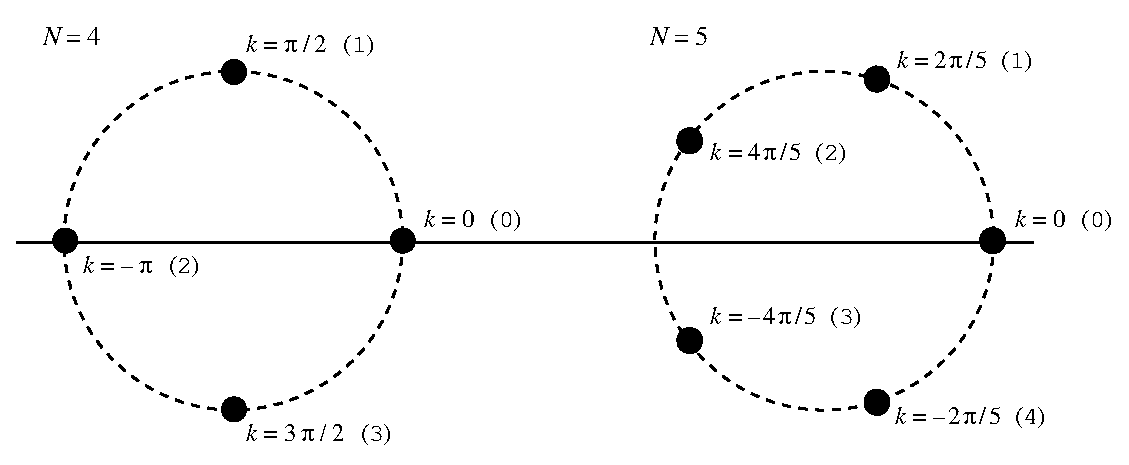
\includegraphics[width=5.5in]{eigsfig.eps}}
\end{center}

As can be seen in the diagram above, the eigenvalues can be divided
into ``general'' values of $k$ which occur in pairs ($k$ and $-k$)
and ``special'' values $k=0$ plus $k=\pi$ if $N$ is even. 
If the original Hamiltonian is symmetric (i.e.\ purely real),
then $H_{k}=H_{-k}$.  In favourable cases, the evolution can
then be calculated using only the postive values of $k$ 
(remembering to double the weighting of signals from general $k$),
halving the calculation time for large $N$.  This relationship breaks down
for sample spinning; presumably because the directionality of the rotation 
breaks the relationship between $k$ and $-k$.  There may also be some
possible speedups using the relations between $k$ and $k+\pi$ ($N$ even only). 

At the special values of $k$, $H_k$ is real for real starting Hamiltonians
(at general values of $k$ the symmetrised Hamiltonian is necessarily complex,
albeit hermitian).  Since operations such as diagonalisation are typically
a factor of 3 faster for purely real matrices, this is a useful efficiency
gain, albeit one that becomes less important as $N$ increases.

Although the contents of {\tt CrystalSpec} are generally only
accessible to {\tt CrystalSystem}, there are a couple of member functions
that can be used to interrogate the object:
\begin{description}
\item[List<size\_t> permutation\_vectorH()] returns the permutation
that ``translates'' states by one unit cell.  
\item[ListList<state\_t> linkedstates()] returns the states broken
down into sets linked by the (translation) symmetry. 
\end{description}

The convention  $j=Mc+j'$ is used to relate the ``spatial'' definition
of a spin in terms of unit cell number, $c$, and index within the cell, $j'$
to spin index
within the spin system, $j'$ (the spin system is always ``flat''). The
function {\tt cell\_to\_spin($M$,$c$,$j'$)} should be used to
return $j$ for a given cell and spin index.

Most NMR parameters are defined over the $M$ spins in the unit cell.
Dipolar couplings, however, are defined between the couplings within cell 0
and between cell 0 and the other cells.  The translational symmetry dictates
that the couplings between cells $c_1$ and $c_2$, for example, are identical
to those between cell 0 and cell $c_2-c_1$.  The coupling network must be
cyclic, so cell $N-1$ can be considered as cell $-1$ etc.

\section{Using the {\tt CrystalSystem} object}

The {\tt CrystalSystem} is initialised from a {\tt CrystalSpec}:
\begin{description}
\item[CrystalSystem(CrystalSpec {\it defin})] creates a {\tt CrystalSpec} object for
the complete space of {\it defin} (no $m_z$ blocking).
\item[CrystalSystem(CrystalSpec {\it defin}, {\it bra $m_z$}, {\it ket $m_z$})]
creates a {\tt CrystalSpec} object spanning a given coherence block, specified
in terms of the $m_z$ values of bra and ket sub-spaces.  A {\tt Failed}
exception thrown if the {\tt CrystalSpec} does not use $m_z$ blocking.
\end{description}

Once the object is defined, it can then be used to generate spin 
operators.  Its use differs from typical
spin-operator generators such as {\tt spin\_system} and {\tt spinhalf\_system}
in the following ways:
\begin{itemize}
\item Rather than return a single matrix, most functions return
the complete manifold for the $k$ states under consideration (as set up
in the {\tt CrystalSpec}).  This is the most efficient way to generate
the spin operators, but other functions allow operators to be calculated
for specific values of $k$, which is useful if memory is tight.

\item Special attention is required when there are less than two states
in the relevant $k$ subspace.  In normal calculations, these cases are
generally obvious and easily accounted for.  In periodic calculations
using $m_z$ blocking, however, small subspaces occur quite frequently and it is useful
to handle them efficiently.  For example, the single state of maximum (or
minimum) $m_z$ generates trivially one state of $k=0$ only.  

\item The homonuclear dipolar coupling Hamiltonian requires special attention.
Normally this is constructed by summing product operator expressions
for all the spin pairs.  This is not practical for large (or even medium)
sized problems.  Instead special functions construct the symmetrised
dipolar coupling Hamiltonian from a specification of the coupling network.
The other spin Hamiltonians do not require special treatment and
can be constructed from spin operators relatively efficiently.
 
\end{itemize}

The simple spin operator functions are
\begin{description}
\item[I(List<cmatrix>\&, $n$, {\it op})] calculates the symmetrised
operator, where $n$ is the spin index $0$ to $MN-1$ (although only
the index modulo $N$ is significant), and {\it op} is {\tt 'x'}, {\tt 'y'}
etc.  The destination is a list of complex matrices, where matrix 0
corresponds to $k=0$ etc.  If a particular $k$ value is not represented
in the selected sub-space, the corresponding matrix will be ``undefined''.
Sub-spaces of size 1 are not treated specially.
\item[I(cmatrix\&,$n$,{\it op},$k$)] returns the spin operator for the specified $k$.
The function above should be used whenever all the eigenvalue blocks are
needed; this function is useful for large problems where there is insufficient
memory to work with all the $k$ states at the same time.
\item[F(List<cmatrix>\&, {\it op})] calculates a symmetrised sum operator (over all spins).
\item[F(List<cmatrix>\&, char* {\it label},{\it op})] restricts the summation to a particular nucleus type.
\item[F(cmatrix\&, {\it op}, $k$) {\rm and} F(cmatrix\&, char* {\it label}, {\it op}, $k$)] calculate a symmetrised sum operators for a given $k$ eigenvalue.
\item[ListList<double> diag\_Iz($n$)] returns a $z$ operator in
``diagonal form''.  The result is a {\tt ListList} rather than the
less efficient {\tt List< List<double> >}.  {\tt result(0)}, for example,
is a {\tt BaseList<double>} corresponding to $k=0$.
\end{description}
There are also more basic {\tt mla} functions that can be used to 
accumulate (scaled) spin operators efficiently.
N.B.\ The spin operator functions use temporary workspace within the {\tt CrystalSystem}
object, hence a multi-threaded calculation should not share
{\tt CrystalSystem} objects, but rather each thread should use its own (the overhead
is tiny).

Because the $z$ operators can be stored compactly, it makes sense
to calculate these once at the start of the calculation.  Full spin operators
are generally too large to be kept around and must be generated as needed.

The following functions calculate symmetrised (homonuclear) dipolar Hamiltonians.
In static problems, the coupling network is specified by a $M \times MN$  \rmx\, $\bs{d}$,
where $d_{ij}$ is the dipolar coupling between spin $i$ of unit cell``zero'' and
spin $j= M c + j'$ ($c$ is the unit cell, $j'$ is the index within the unit cell). 
Note that the coupling network defined by $\bs{d}$ must be cyclic (as explained above).  Couplings that are identically zero are ignored.
%Functions that deal with Hamiltonians treat singly-degenerate matrix blocks
%separately, since $1 \times 1$ matrices are extremely inefficient to handle 
%and they are usually special cases.

In spinning problems, it is necessary to provide a rank 2 tensor (as a {\tt space\_T}) to define the strength and orientation of the dipolar interaction.
Rather than return a {\tt List<cmatrix>}, the functions create a {\tt List< Tensor<cmatrix> >} i.e.\ for each value of $k$, the Hamiltonian is defined in terms
of components $H^{(l)}_m$ which transform as rank $l$ spherical tensors ($l$ is always 2).
Note that the functions also take the $\bs{d}$ matrix in addition to the spatial
tensor information, where the $d_{ij}$ are just used to determine whether a
particular interaction is to be included or not.

\begin{description}
\item[sym\_Hdipolar(List<cmatrix>\& $H$, List<double>\& $h$, rmatrix $\bs{d}$)] creates
the symmetrised dipolar coupling Hamiltonian defined by coupling network $\bs{d}$.
If the coupling is heteronuclear (as defined by the initial {\tt spinhalf\_system}), only the
secular components of the dipolar Hamiltonian are used.
\emph{If the $k$ block contains a
single state, the symmetrised element is stored in $h(k)$ of the $h$ vector
and the corresponding $H$ matrix will be undefined.}

\item[sym\_Hdipolar(cmatrix\& $H$, double\& $h$, $\bs{d}$, $k$)] stores the dipolar Hamiltonian for a particular $k$ value in $H$ or $h$.  This function is for large
problems where memory is insufficient to handle all $k$ values at the same time.
\item[double sym\_Hdipolar\_element($\bs{d}$)] handles the special case where the Hilbert space contains
a single state (i.e.\ {\tt rows()} is 1).  It returns the single element of the dipolar Hamiltonian.
\item[sym\_Hdipolar(List< Tensor<cmatrix> >\& $H$, List<space\_T>\& $h$,$\bs{d}$, Matrix<space\_T> $\bs{D}$)] calculates the Fourier components $H^{l}_m$ of the dipolar
Hamiltonian under spinning\footnote{By default, magic angle spinning is assumed for the sake of efficiency, but this can be easily changed}.  Single-element $k$ blocks are stored in the simple {\tt space\_T}, $h$.
\item[sym\_Hdipolar(Tensor<cmatrix>\& $H$, space\_T\& $h$,$\bs{d}$,$\bs{D}$,$k$)] calculates the Fourier components for a single value of $k$.
\item[complex sym\_Hdipolar\_element($\bs{d}$,$\bs{D}$,$k$)] return the single element of
the dipolar Hamiltonian for the special case of a Hilbert space consisting of a single state.
\end{description}

Other member functions of {\tt CrystalSystem}
\begin{description}
\item[isdiagonal()] returns {\tt true} if the Hilbert space is diagonal (always true
if no $m_z$ blocking).
\item[rows() \& cols()] return the dimensions of the Hilbert space.
\item[rows($k$) \& cols($k$)] return the dimensions of a particular eigenvalue block
of the symmetrised space. 
\end{description}

\section{How it works}

The mathematics of the symmetrisation is essentially limited to
Equation~(\ref{Vmatrix}).  The complications lie in the book-keeping of
combining the right states and putting the result in the right place.
The spin operator generating functions use a {\tt CrystalSystem\_iterator} to
iterate over each set
of symmetry-linked states, generating elements of the symmetrised operators.
For instance, if sets $i$ and $j$ both contain $N$ states, the $N \times N$
block of the original operator is first calculated and then transformed
(by the {\tt symmetrise} internal functions)
to generate a diagonal vector containing $N$ elements corresponding to the
$N$ values of $k$.  These are then placed into the $i,j$ elements of the
output matrix blocks (by the {\tt place} functions).  Things are complicated somewhat by the presence (for
non-prime $N$) of sets that contain less than $N$ states, but this is 
essentially book-keeping.

Various special cases are considered to make the whole thing go faster:
\begin{itemize}
\item Diagonal spin operators: only diagonal $i,i$ blocks need be considered
and the maths can be further simplified.
\item For simple spin operators, it is more efficient to calculate the symmetrised
matrix elements directly rather than transform a fairly sparse matrix.
\item In the dipolar coupling Hamiltonian, it is not necessary to consider 
all the $MN(MN+1)/2$ couplings.  The symmetry allows us to consider 
just the couplings from (and within) cell 0 ($\sim M^2N$) and simply multiply the
symmetrised Hamiltonian by $N$.
\item $k=0$ can be handled specially.  If the original matrix is real, the $k=0$ block is also real.  In this implementation, the results are always stored
in complex matrices which need to be turned into real versions before
functions such as {\tt symmetric\_eigensystem} can be used.
The is somewhat wasteful, but the wastage is $O(n^2)$ compared to $O(n^3)$
for the major time-takers.
\end{itemize}

Profiling a program that uses {\tt crystal.h} shows
the vast majority of the time is spent in diagonalisation, matrix multiplication etc.,
i.e.\ the overhead of symmetrisation is not significant.


\end{document}
